\chapter{Definição e planejamento da proposta} \label{cap:proposta}

 A seção \ref{requirements} apresenta os requisitos identificados para a solução.
 A seção \ref{architecture} apresenta a descrição da arquitetura definida para a solução.

\section{Requisitos da solução} \label{requirements}

    Considerando as necessidades do ``Empurrando Juntos'',
    foram identificados requisitos funcionais e não funcionais da aplicação,
    que são apresentados a seguir.

    \subsection*{Requisitos Funcionais} \label{functional_requirements}

    Uma avaliação do escopo da plataforma ``Empurrando Juntos'' permitiu o levantamento de \textit{features} desejadas do sistema e,
    consequentemente, alguns requisitos associados, que foram sumarizados na listagem abaixo.
    
    É importante salientar que os requisitos identificados foram levantados no trabalho de \citeonline{empurrandojuntos}
    e neste trabalho somente foi realizada a tradução do requisito para a forma de histórias de usuários, que
    foram documentadas como \textit{issues} no repositório
    da aplicação\footnote{\href{https://gitlab.com/pentano}{https://gitlab.com/pentano}}.

    \begin{itemize}
	\item \textbf{Feature}:  Gerenciamento de Usuário
	    \begin{itemize}
		\item Como usuário, gostaria de me cadastrar na plataforma para poder participar das discussões.
		\item Como usuário, gostaria de acessar a plataforma utilizando minha conta da própria plataforma para ter acesso às discussões.
		\item Como usuário, gostaria de acessar a plataforma utilizando minha conta do Facebook para não ter que preencher muitos dados e poder ter acesso rápido às discussões.
		\item Como usuário, gostaria de alterar meus dados cadastrais para manter minhas informações atualizadas.
	    \end{itemize}
	    
	\item \textbf{Feature}: Gerenciamento de Conversa
	    \begin{itemize}
		\item Como usuário, gostaria de criar uma conversa para iniciar uma discussão sobre um tema de minha escolha. 
		\item Como usuário, gostaria de editar minha conversa para corrigir possíveis erros no texto. 
		\item Como usuário, gostaria de excluir minha conversa para encerrar a discussão apresentada.
	    \end{itemize}
	    
	\item \textbf{Feature}: Gerenciamento de Comentário
	    \begin{itemize}
		\item Como usuário, gostaria de criar um comentário em uma conversa para expressar minha opinião sobre o assunto da conversa. 
		\item Como usuário, gostaria de editar meu comentário em uma conversa para corrigir possíveis erros no texto. 
		\item Como usuário, gostaria de excluir meu comentário em uma conversa para deixar de expressar minha opinião naquela conversa. 
	    \end{itemize}
	    
	\item \textbf{Feature}: Agrupamento de usuários
	    \begin{itemize}
		\item Como usuário, gostaria de votar em um comentário para expressar minha opinião sobre o conteúdo daquele comentário.
		\item Como usuário, gostaria de visualizar os grupos formados em uma conversa para ter uma visão geral das pessoas na discussão.
	    \end{itemize}
    \end{itemize}
%     \begin{table}[h!]
%     \centering
%     \caption{Requisitos funcionais de alto nível da aplicação.}
%     \label{tab:requisitos}
%     \resizebox{\columnwidth}{!}{
%       \begin{tabular}{@{}cl@{}}
%       \toprule
%       \textbf{Característica}                      & \multicolumn{1}{c}{\textbf{Requisito}}                                                                                                \\ \midrule
%       \multirow{5}{*}{Gerenciamento de Usuário}    & O sistema deve permitir o cadastro de usuários                                                                                        \\
% 						  & O sistema deve permitir a alteração de usuários                                                                                       \\
% 						  & \begin{tabular}[c]{@{}l@{}}O sistema deve permitir a autenticação de usuários \\ cadastrados na plataforma\end{tabular}			\\
% 						  &  \begin{tabular}[c]{@{}l@{}}O sistema deve permitir a autenticação de usuários \\ cadastrados no Facebook\end{tabular}                     \\ \midrule
%       \multirow{3}{*}{Gerenciamento de Conversa}   & O sistema deve permitir o cadastro de conversas                                                                                       \\
% 						  & O sistema deve permitir a alteração de conversas                                                                                      \\
% 						  & O sistema deve permitir a exclusão de conversas                                                                                       \\ \midrule
%       \multirow{4}{*}{Gerenciamento de Comentário} & O sistema deve permitir o cadastro de comentários em conversas                                                                        \\
% 						  & O sistema deve permitir a alteração de comentários                                                                                    \\
% 						  & O sistema deve permitir a exclusão de comentários                                                                                     \\ 
% 						  & O sistema deve permitir que o usuário vote em comentários                                                                             \\ \midrule
%       Agrupamento de usuários                      & \begin{tabular}[c]{@{}l@{}}O sistema deve permitir a 
% 						    visualização dos usuários agrupados \\ de acordo com os votos dados\end{tabular} \\ \bottomrule
% 	\end{tabular}
%     }
% 	\end{table}
	  
      
    \subsection*{Requisitos não funcionais}	\label{non_functional_requirements}
    
    O ``Empurrando Juntos'' possui a característica de ser uma aplicação multiplataforma,
    que terá sua própria aplicação \textit{web} e aplicativos nas diversas plataformas existentes,
    o que cria uma necessidade das funcionalidades principais da aplicação serem reutilizáveis
    pelas diversas plataformas que possam existir.
    
    O agrupamento dos usuários geralmente é um processo computacionalmente custoso e recorrente. Por isso, o ``Empurrando Juntos''
    necessita de uma solução que realize esse processamento de forma assíncrona e distribuída, para que a comunicação com
    as aplicações clientes possam ser mais fluidas e que possa haver máquinas dedicadas ao processamento.
    
    Outro aspecto importante para esta aplicação é a questão da manutenibilidade, pois como é um software livre, a solução
    deve ser desenvolvida de uma maneira que seja possível evoluir facilmente pela comunidade.
    
    \subsection*{Suporte tecnológico}
    
    Todos os serviços da API serão providos para a plataforma por meio de uma interface HTTP/HTTPS utilizando o estilo arquitetural REST.
    Para isso, a linguagem Python\footnote{Versão 3.4 - \href{https://www.python.org/download/releases/3.4.0/}{https://www.python.org/download/releases/3.4.0/}} 
    foi definida como tecnologia de implementação da solução proposta, juntamente com os \textit{frameworks}
    Django\footnote{Versão 1.11 - \href{https://www.djangoproject.com/}{https://www.djangoproject.com/}} e 
    Django Rest Framework\footnote{Versão 3.6.3 - \href{http://www.django-rest-framework.org/}{http://www.django-rest-framework.org/}}, 
    utilizando o banco de dados PostgreSQL\footnote{Versão 10.1 - \href{https://www.postgresql.org/}{https://www.postgresql.org/}}.
    A autenticação e autorização das aplicações e seus respectivos usuários serão realizadas por meio de JWT \textit{tokens}.
     
    Para que o agrupamento dos usuários possa ser realizado de forma assíncrona e distribuída, 
    foi utilizada uma plataforma de execução de tarefas assíncronas,
    o Celery\footnote{\href{http://www.celeryproject.org/}{http://www.celeryproject.org/}},
    que é uma aplicação de filas de tarefas assíncronas distribuídas focada em processamento em tempo real.
    O Celery foi escolhido por ser uma aplicação madura, estável, escrita em Python e bem acolhida pela comunidade Python,
    o que a torna de fácil integração com projetos nessa linguagem.
    Como a necessidade do ``Empurrando Juntos'' está mais ligada a operações em tempo real,
    processamento do agrupamento dos usuários à medida que os votos mudam,
    o Celery é adequado para fornecer as funcionalidades necessárias relacionadas ao processamento assíncrono e distribuído.
    
    Para executar as tarefas de forma assíncrona e distribuída, o Celery utiliza um \textit{message broker},
    que é uma plataforma intermediária entre duas aplicações para troca de mensagens,
    para enfileirar e delegar as tarefas para execução. 
    Para este trabalho, o RabbitMQ\footnote{\href{https://www.rabbitmq.com/}{https://www.rabbitmq.com/}}
    foi escolhido como \textit{message broker} por ser uma aplicação madura, tolerante a falhas e performática
    (escrito em Erlang \footnote{\href{https://www.erlang.org/}{https://www.erlang.org/}}),
    com armazenamento persistente das filas, suporte a \textit{backup}, suporte à \textit{plugins},
    possibilidade de formação de \textit{clusters} para alta disponibilidade,
    boa documentação e por ser \textit{open source}.
    Além disso, o RabbitMQ é o \textit{message broker} padrão do Celery, contando com uma boa integração com a ferramenta.
    
    Em relação à manutenibilidade da aplicação, considerando as tecnologias escolhidas,
    foram definidas os seguintes padrões para o desenvolvimento da aplicação:
    utilização do PEP8\footnote{Folha de estilos PEP8. Disponível em \href{https://www.python.org/dev/peps/pep-0008/}{https://www.python.org/dev/peps/pep-0008}.}
    como folha de estilos, por ser a folha de estilos oficial da linguagem Python,
    e a utilização da especificação JSON API\footnote{Especificação JSON API. Disponível em \href{http://jsonapi.org/}{http://jsonapi.org}.}
    para formatação das respostas da API, por ser uma especificação consolidada e bem documentada que possui padrões que
    se adequam às restrições do estilo REST.
    
\section{Planejamento do trabalho}

    Para a execução do trabalho foi utilizada uma abordagem ágil, onde os requisitos foram alocados em 6 iterações de duas semanas e
    este planejamento pode ser visto na Figura \ref{fig:cronograma}.
    
    \begin{figure}[h!]
      \centering
      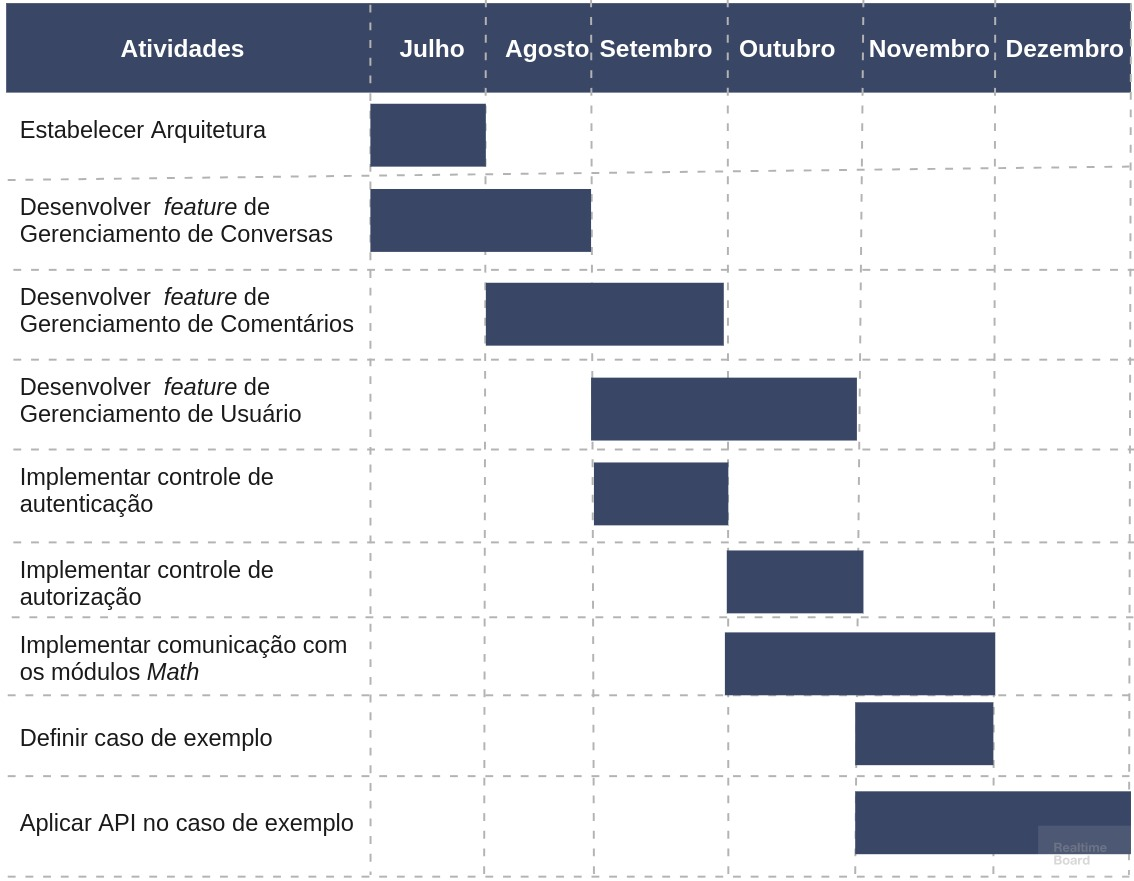
\includegraphics[scale=0.3]{figuras/cronograma.jpg}
      \caption{Cronograma de iterações de desenvolvimento}
      \label{fig:cronograma}
    \end{figure}
